 \begin{minipage}{\linewidth}
      \begin{minipage}{0.45\linewidth}
          \begin{figure}[H]\centering
		\caption{pH set means, class 1}
           	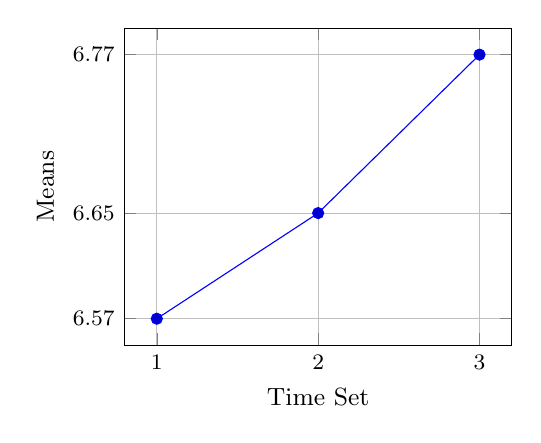
\begin{tikzpicture}
		\begin{axis}[xlabel = Time Set,ylabel = Means,small,xtick = {1,2,3}, ytick=data, grid=both]
		\addplot coordinates{(1,6.57) (2,6.65) (3,6.77)};
		\end{axis}
	\end{tikzpicture}
	\label{fig:ANOVApH1}
          \end{figure}
      \end{minipage}
      \hspace{0.05\linewidth}
      \begin{minipage}{0.45\linewidth}
          \begin{figure}[H]\centering
		\caption{pH set means, class 2}
 		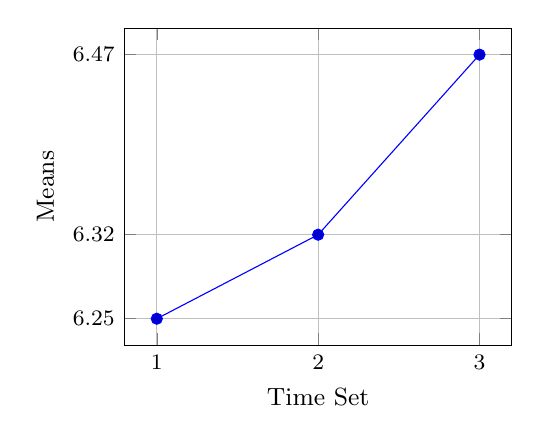
\begin{tikzpicture}
		\begin{axis}[xlabel = Time Set,ylabel = Means,small,xtick = {1,2,3}, ytick=data, grid=both]
		\addplot coordinates{(1,6.25) (2,6.32) (3,6.47)};
		\end{axis}
	\end{tikzpicture}
	\label{fig:ANOVApH2}
          \end{figure}
      \end{minipage}
   \hspace{0.05\linewidth}
      \begin{minipage}{0.45\linewidth}
          \begin{figure}[H]\centering
	\caption{pH set means, class 3}
        	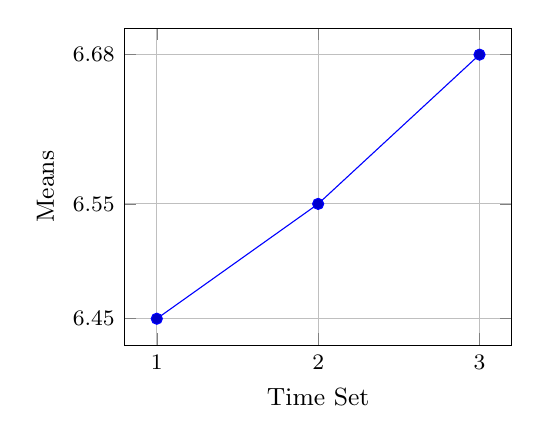
\begin{tikzpicture}	
		\begin{axis}[xlabel = Time Set,ylabel =Means,small,xtick = {1,2,3}, ytick=data, grid=both]
		\addplot coordinates{(1,6.45) (2,6.55) (3,6.68)};
		\end{axis}
	\end{tikzpicture}
	\label{fig:ANOVApH3}
          \end{figure}
      \end{minipage}
   \hspace{0.05\linewidth}
      \begin{minipage}{0.45\linewidth}
          \begin{figure}[H]\centering
	\caption{pH set means, class 4}
        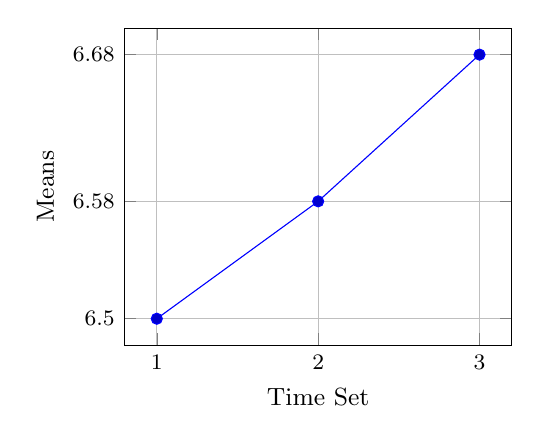
\begin{tikzpicture}
		\begin{axis}[xlabel = Time Set,ylabel = Means,small,xtick = {1,2,3}, ytick=data, grid=both]
		\addplot coordinates{(1,6.50) (2,6.58) (3,6.68)};
		\end{axis}
	\end{tikzpicture}
	\label{fig:ANOVApH4}
          \end{figure}
      \end{minipage}
   \hspace{0.05\linewidth}
      \begin{minipage}{0.45\linewidth}
          \begin{figure}[H]\centering
	\caption{pH set means, class 5}
        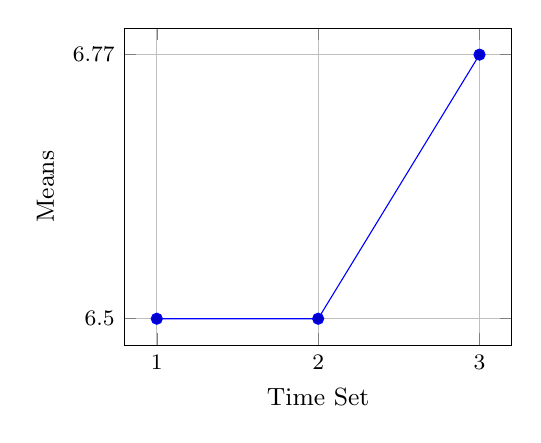
\begin{tikzpicture}
		\begin{axis}[xlabel = Time Set,ylabel =Means,small,xtick = {1,2,3}, ytick=data, grid=both]
		\addplot coordinates{(1,6.50) (2,6.50) (3,6.77)};
		\end{axis}
	\end{tikzpicture}
	\label{fig:ANOVApH5}
          \end{figure}
      \end{minipage}
   \hspace{0.05\linewidth}
      \begin{minipage}{0.45\linewidth}
          \begin{figure}[H]\centering
	\caption{pH set means, class 6}
        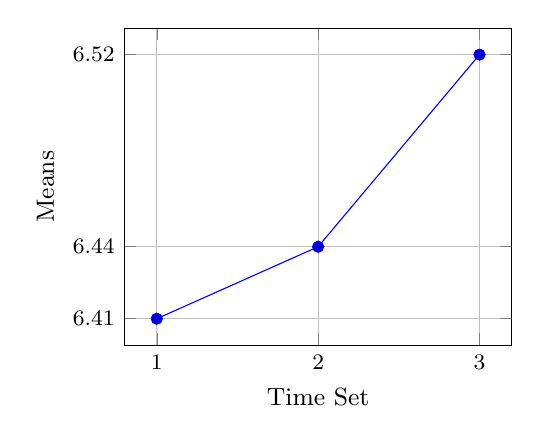
\begin{tikzpicture}	
		\begin{axis}[xlabel = Time Set,ylabel =Means,small,xtick = {1,2,3}, ytick=data, grid=both]
		\addplot coordinates{(1,6.41) (2,6.44) (3,6.52)};
		\end{axis}
	\end{tikzpicture}
	\label{fig:ANOVApH6}
          \end{figure}
      \end{minipage}
  \end{minipage}
  
%  \newpage
%\section{Figures}
%\subsection{Single figures}
%For more information, check: \href{http://en.wikibooks.org/wiki/LaTeX/Floats,_Figures_and_Captions}{http://en.wikibooks.org/wiki/LaTeX/Floats,\_Figures\_and\_Captions}
%\begin{verbatim}
    %\begin{figure}[t for top, b for bottom, h for here, ! to force placement]
        % Requires \usepackage{graphicx}
        %\centering % center the figure
        %\includegraphics[width=5in or 127mm etc...]{figure-name}\\
        %\caption{figure caption}\label{figure label}
    %\end{figure}
%\end{verbatim}
%\begin{figure}[h!]
  % Requires \usepackage{graphicx}
  %\centering
  %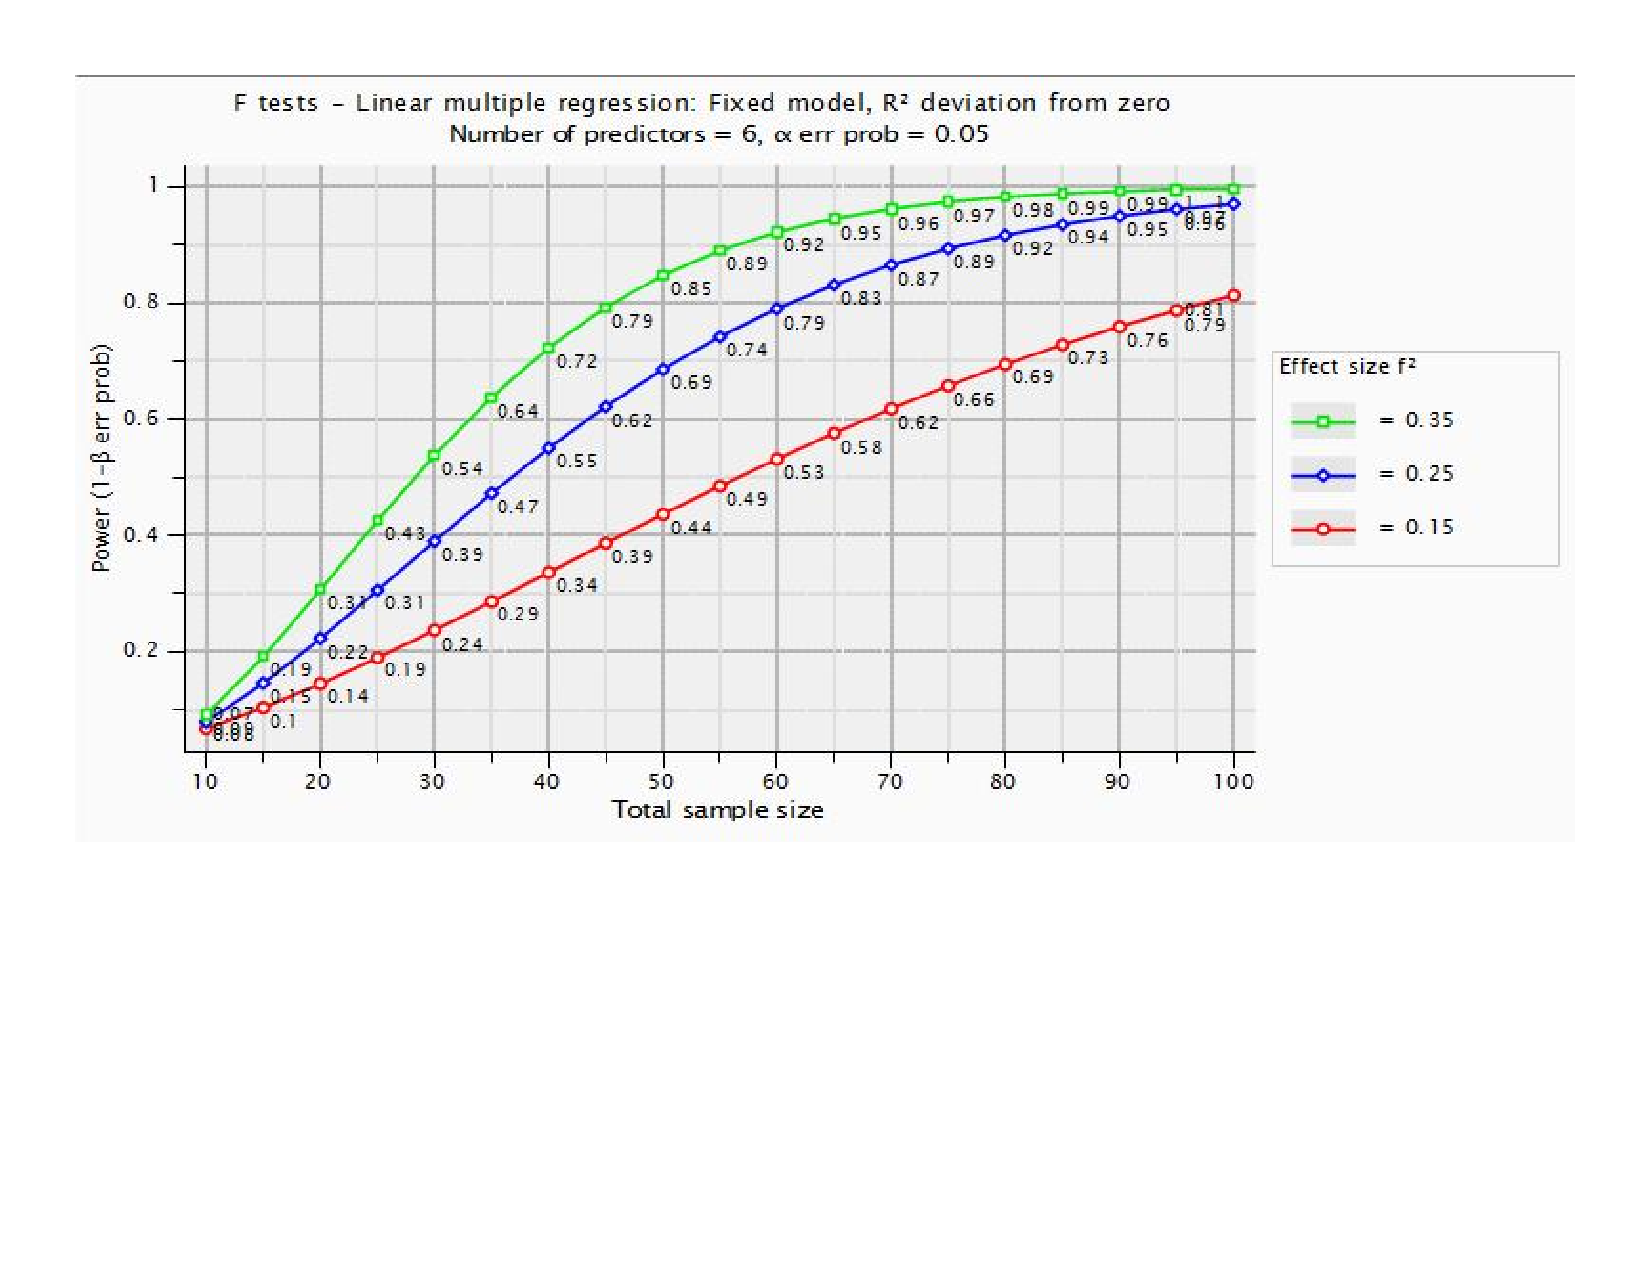
\includegraphics[width=3in]{pH}\\
  %\caption{Sample caption.}\label{label}
%\end{figure}
%\newpage
%\subsection{Multipart figures}
%For multipart figures, you need to use the package "subfig". here's an example
%\begin{verbatim}
%\begin{figure}
    %\centering
    %\subfloat[figure a]{\label{fig:figure-a} \includegraphics[width=w]{fig02a}}
    %\subfloat[figure b]{\label{fig:figure-b} \includegraphics[width=w]{fig02b}}
	%\subfloat[figure d]{\label{fig:figure-d} 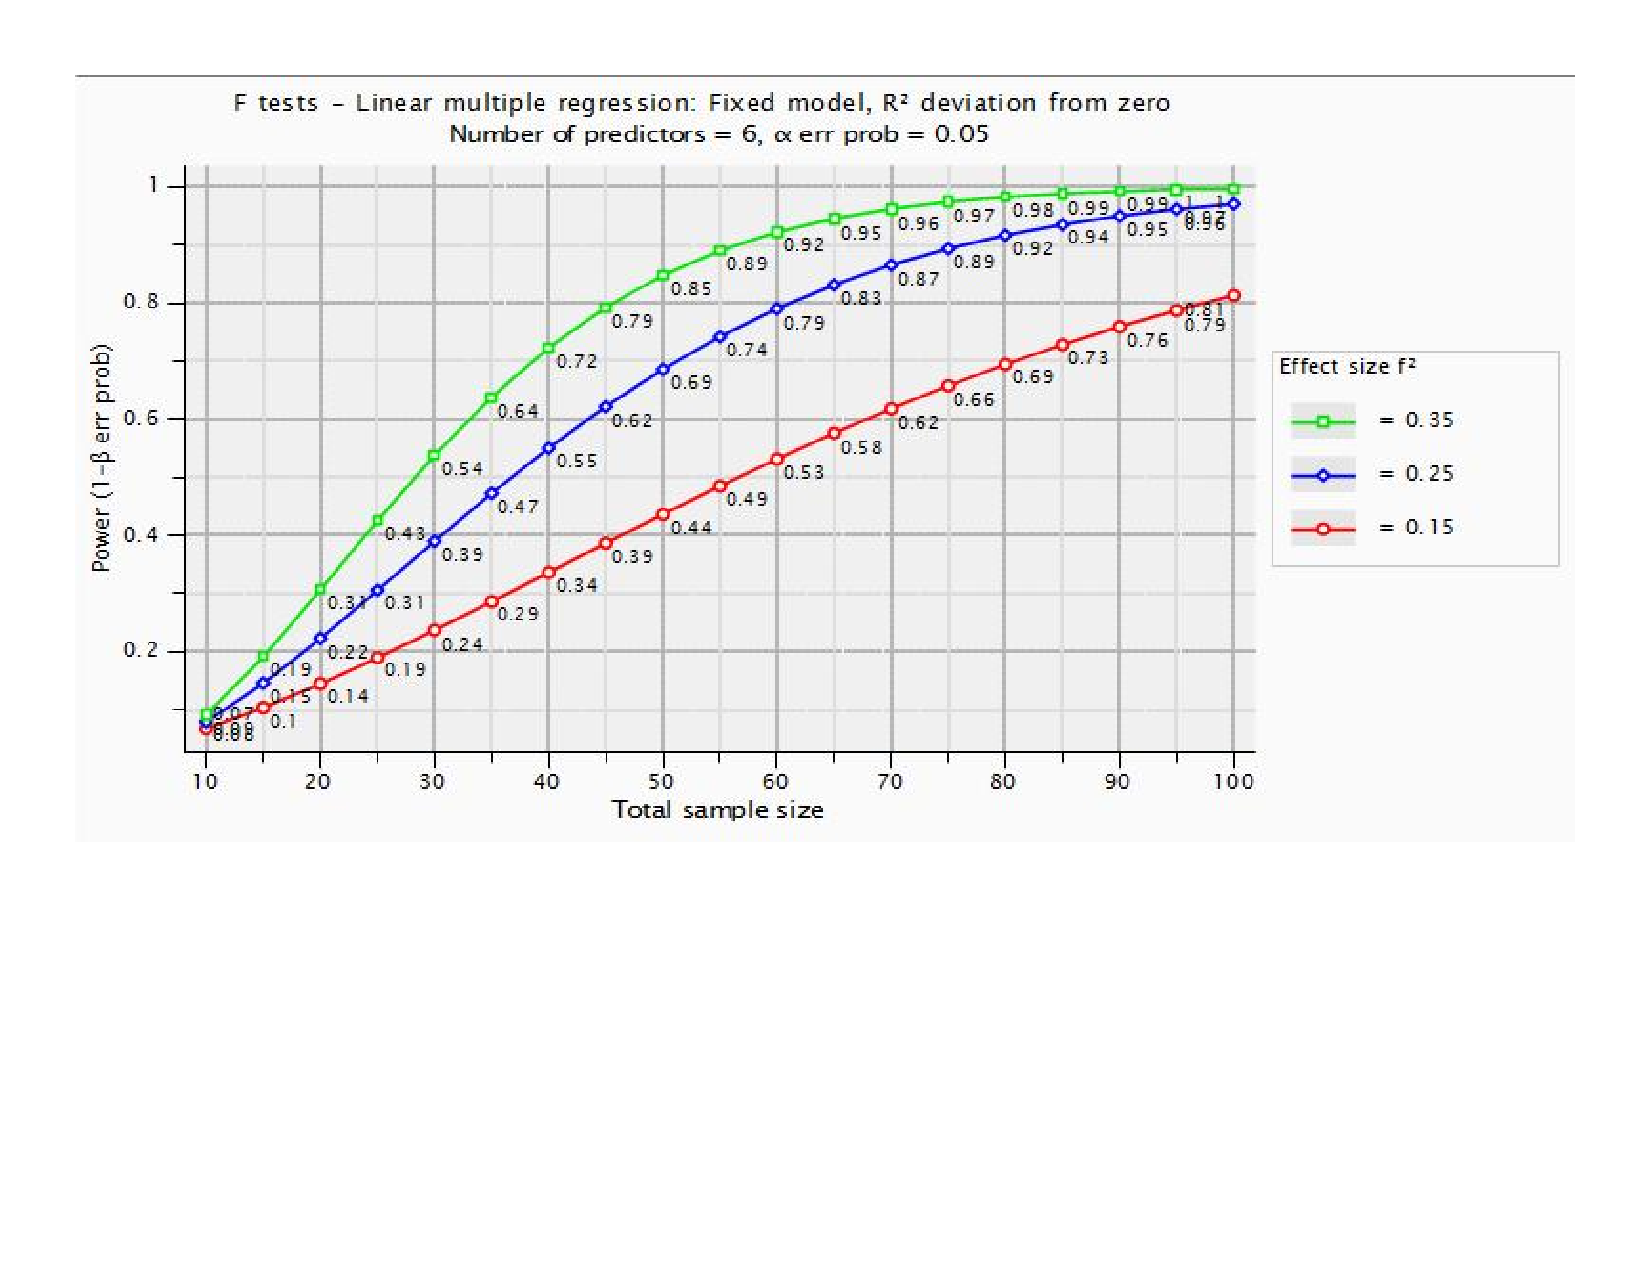
\includegraphics[width=w]{pH}}
    %\caption{Sample of a multipart figure} \label{fig:multipart-figure}
%\end{figure}
%\end{verbatim}
%\begin{figure}[h!]
    %    \centering
        %\subfloat[Circle]{\label{fig:figure-a}
\includegraphics[width=1.1in]{fig02a-circle}}
        %\subfloat[Rectangle]{\label{fig:figure-b}
\includegraphics[width=1.1in]{fig02b-rectangle}}
        %\subfloat[Cube]{\label{fig:figure-c}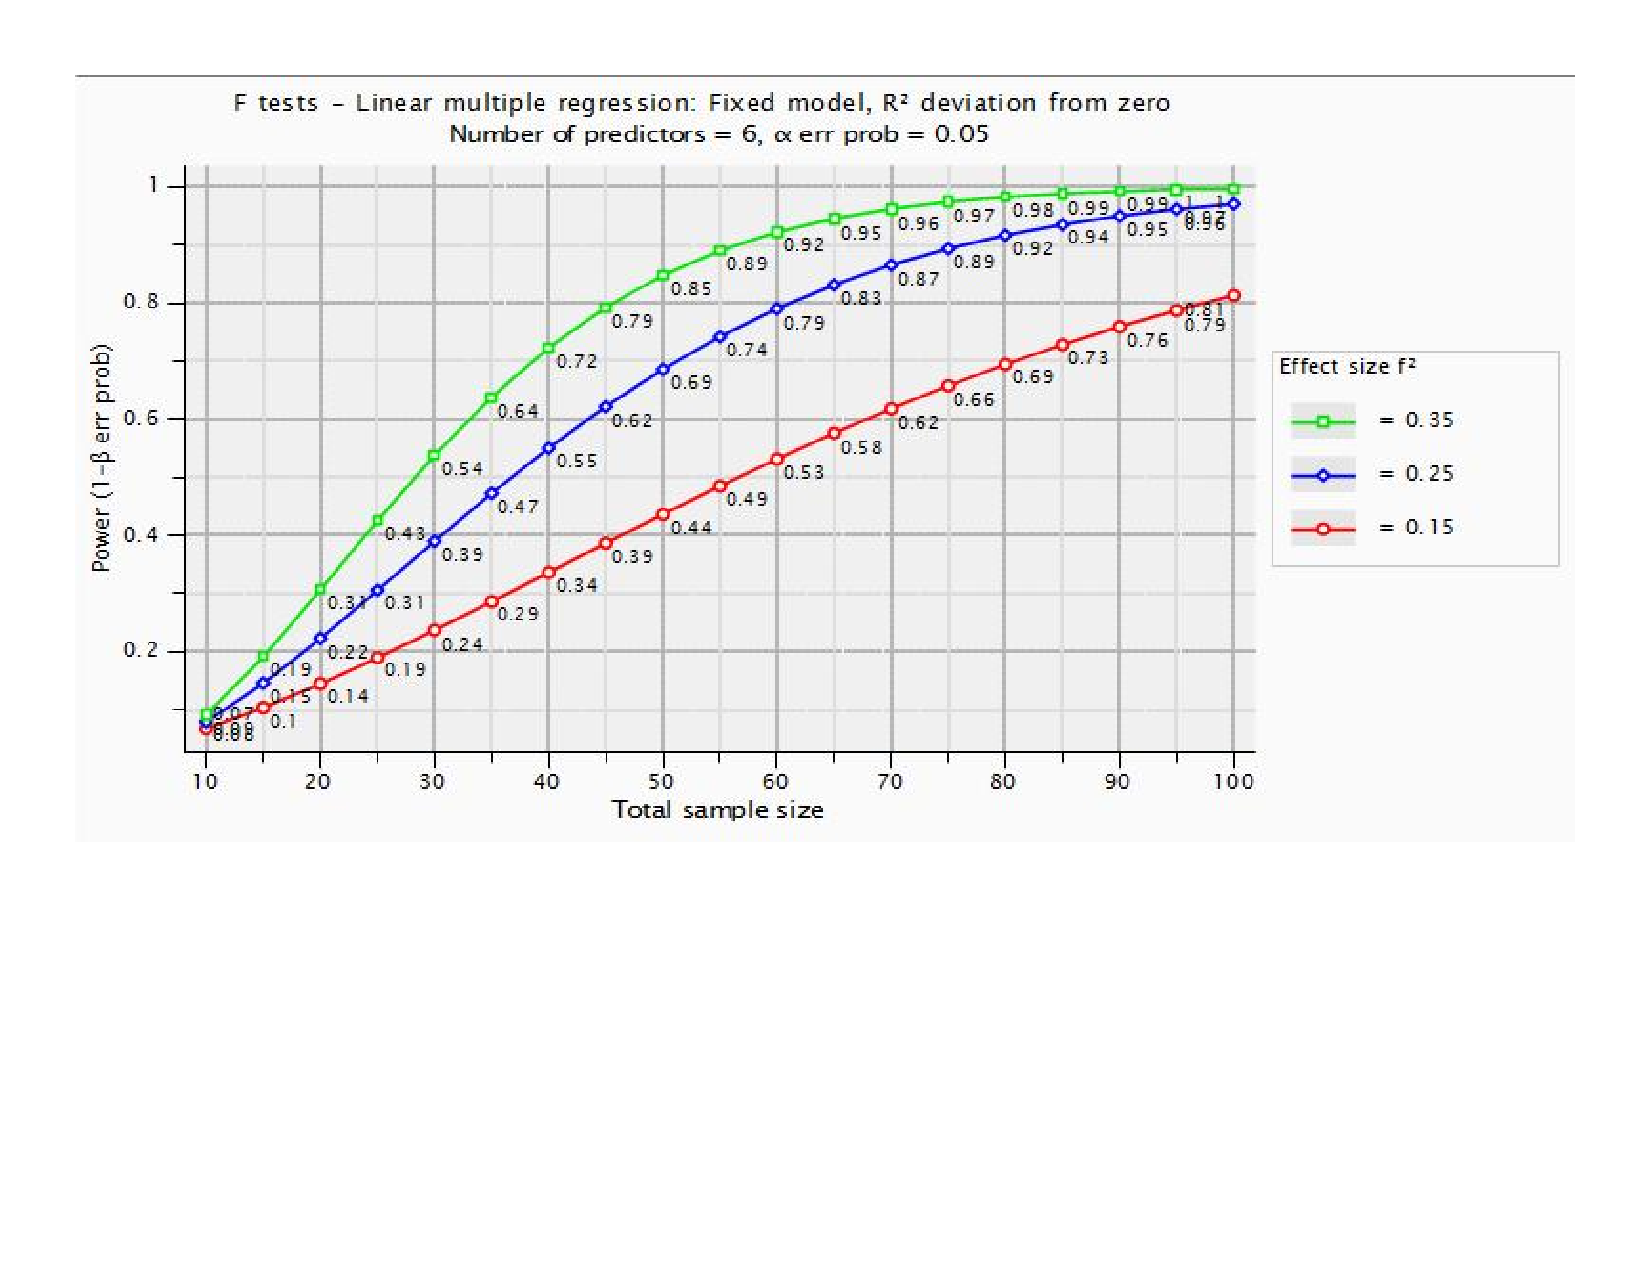
\includegraphics[width=1.1in]{pH}}
        %\caption{Geometric shapes.}
        %\label{fig:multipart-figure}
%\end{figure}
%To add some space between the figures above, one can use the usual spacing commands such as ``qquad''
%\begin{figure}[h!]
    %    \centering
        %\subfloat[Circle]{\label{fig:figure-a}
\includegraphics[width=1.1in]{fig02a-circle}} \qquad
        %\subfloat[Rectangle]{\label{fig:figure-b}
\includegraphics[width=1.1in]{fig02b-rectangle}}\qquad
        %\subfloat[Cube]{\label{fig:figure-c}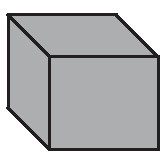
\includegraphics[width=1.1in]{fig02c-cube}}\qquad
        %\caption{Geometric shapes.}
        %\label{fig:multipart-figure}
%\end{figure} 